% 独立版式样张：内容仅用于观察排版，不是赛题解答。
\PassOptionsToPackage{fontset=fandol}{ctex}
\documentclass[withoutpreface,notoc,bwprint]{cumcmthesis}
% 使用 Sustainable-Enjoyment 模板本身的视觉样式。
% 旧样式已归档至 archive/legacy-template-files/cumcm2026.sty，不再加载，
% 避免覆盖上游标题、间距与图表样式。
\usepackage[super,numbers,sort&compress]{natbib}
% Noto Sans Mono 覆盖代码中的摄氏度等符号；中文仍由 ctex 字体回退处理。
\newfontfamily\CumcmCodeFont{NotoSansMono-Regular.ttf}
\newcolumntype{C}{>{\centering\arraybackslash}X}
\newcolumntype{R}{>{\raggedleft\arraybackslash}X}
\newcolumntype{L}{>{\raggedright\arraybackslash}X}
\BeforeBeginEnvironment{tabular}{\zihao{-5}}
% 给上游代码行号和外框留出内侧空间，防止侵入25mm页边距。
\lstset{basicstyle=\CumcmCodeFont\small,xleftmargin=12pt,xrightmargin=4pt}
\pagestyle{plain}
\hypersetup{pdfauthor={},pdfsubject={CUMCM 2026}}
\newcommand{\CumcmAIUsed}[1]{\section*{AI工具使用声明}本参赛队在竞赛过程中使用了AI工具，主要用于#1，详细使用情况见支撑材料中的《AI工具使用详情.pdf》。}
\newcommand{\CumcmAINotUsed}{\section*{AI工具使用声明}本参赛队在竞赛过程中未使用任何AI工具。}

% 正式图片优先，其次是可编辑图源和上游模板示例图片。
\graphicspath{{figures/final/}{figures/source/}{figures/}}

% 常用数学记号可在此集中定义，避免各章节重复声明。
\newcommand{\dif}{\mathop{}\!\mathrm{d}}

\title{数学建模论文排版样张与使用说明}
\begin{document}
\maketitle
\thispagestyle{plain}
\begin{abstract}
本文件用于展示现成模板在连续中文正文、数学公式、三线表和插图共同出现时的版面效果。本文采用 Sustainable-Enjoyment 的数学建模论文模板，保留其标题层级、段落间距、图表题注与代码环境。文中的数学关系为基础示例，配图来自模板仓库，不包含任何本届赛题分析或实测结果。本文件仅供选择版式，不能作为参赛论文提交。

\textbf{在内容组织方面，}示例将叙述、符号解释与公式放在相邻位置，使读者能够先理解研究对象，再阅读数学表达。章节数量由实际任务决定，不要求每个问题都采用完全相同的段落结构。符号表仅集中列出反复使用的变量，临时变量在首次出现时直接解释。

\textbf{在图表呈现方面，}表格用于承载需要精确比较的信息，插图用于呈现形态与结构。表题置于表格上方，图题置于图形下方，并通过交叉引用与正文衔接。示例保留模板原有三线表与单图排版，便于直接复制到实际论文中；正式图表应替换为团队计算得到、能够复现的内容。

\textbf{在模型表述方面，}以一阶衰减方程演示行内符号、独立公式、编号和求解说明。先定义状态量与参数，再列出方程及其解析解，最后解释初值和参数对解的作用。该例仅用于观察数学符号与中文正文的混排效果，不代表对未来赛题的模型推荐。

\textbf{在交付结构方面，}摘要单独成页，正文接续排版，不插入目录。AI工具使用声明安排在参考文献之前，附录包含文件清单与完整示例程序。字号、字体和行距延续上游模板；页边距及摘要页编号按已公布的2026年格式规范核对。竞赛期间新增的图表、引用和程序仍需随内容逐项复核。

\keywords{版式样张\quad 数学表达\quad 三线表\quad 交叉引用}
\end{abstract}

\section{问题重述与内容组织}
本样张解决的是排版预览问题：在具有实际段落密度的页面中，检查标题、正文、数学式和图表之间的比例是否协调。上一次空白骨架只有连续标题，无法反映成文后的阅读体验，因此这里提供完整的示例段落。所有示例内容与正式论文分开存放，写作时从主文档入口填写实际研究内容。

正文应围绕需要解决的问题展开。通常先交代研究对象、可用数据和约束，再介绍模型、求解过程及结果解释。若多个问题共用数据处理步骤，可将其单独组织；若某一步只服务于一个问题，则放入对应章节。这样的组织方式能够减少重复，并让读者顺着证据理解结论。

\section{符号与数学表达}
\subsection{符号定义}
以衰减过程为例，设状态量随时间变化，变化速率与当前状态成正比。为明确公式含义，先在表\ref{tab:symbols}中列出本例使用的符号。单位一栏采用一般性记号，正式论文应替换为相应物理单位。
\begin{table}[htbp]
\centering
\caption{示例方程中的符号与含义}
\label{tab:symbols}
\begin{tabularx}{\textwidth}{CLC}
\toprule
符号 & 含义 & 单位\\
\midrule
$t$ & 自初始时刻起经过的时间 & 时间单位\\
$x(t)$ & 时刻 $t$ 的状态量 & 状态单位\\
$x_0$ & 初始状态量 & 状态单位\\
$k$ & 衰减率，且 $k>0$ & 时间单位$^{-1}$\\
\bottomrule
\end{tabularx}
\end{table}

\subsection{方程建立与求解}
在上述示例假设下，状态量满足式\eqref{eq:decay}。公式编号沿正文连续生成，引用编号自动更新，避免章节增删后手动改号。
\begin{equation}
\frac{\dif x}{\dif t}=-kx,\qquad x(0)=x_0.
\label{eq:decay}
\end{equation}
对 $x_0>0$ 的情形分离变量并积分，可得解析解。将其代回原方程，可以同时核对微分关系与初始条件：
\begin{equation}
x(t)=x_0\exp(-kt),\qquad t\geq 0.
\label{eq:solution}
\end{equation}
式\eqref{eq:solution}表明，初值决定曲线起点，参数 $k$ 决定衰减速度。这里没有给出拟合参数或误差指标，因为示例没有使用观测数据。实际建模时，应补充参数估计方法、数据来源和误差检验，并将计算结果与文字结论对应。

\section{图形呈现与结果说明}
图\ref{fig:upstream}直接使用模板仓库自带示例图，目的在于展示单图宽度、图题和正文的组合。它与前文衰减方程无关。论文中的正式图应具有清楚的坐标、单位与图例；图注说明图中表达了什么，正文进一步解释其对研究问题的意义。
\begin{figure}[htbp]
\centering
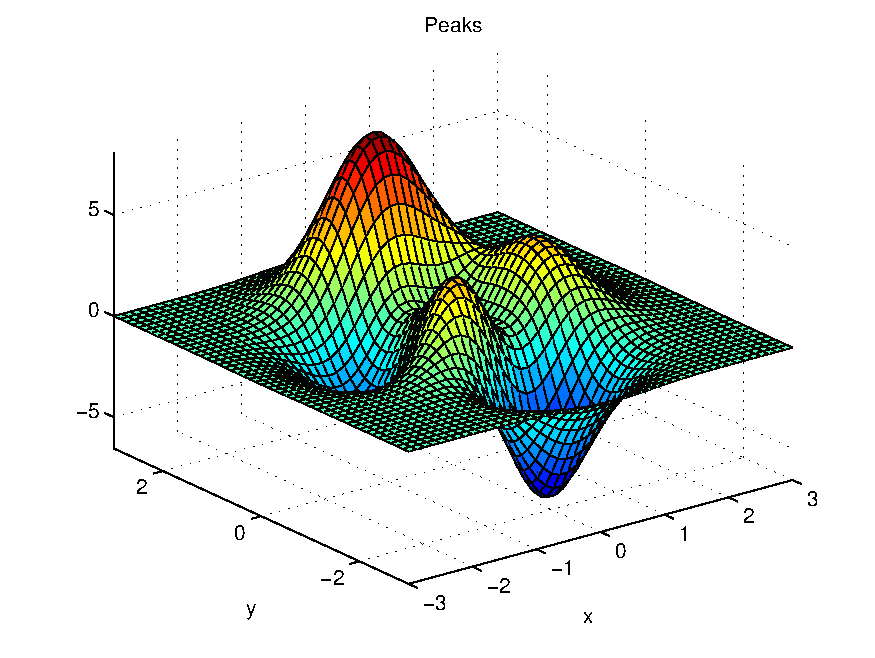
\includegraphics[width=0.7\textwidth]{preview/upstream-example.pdf}
\caption{上游模板自带插图（仅作版式演示）}
\label{fig:upstream}
\end{figure}
阅读一幅结果图时，应能够从正文找到数据来源、处理过程和关键观察。若图中呈现多个方案，说明比较条件是否一致；若展示拟合曲线，明确散点与模型输出的区别。排版提供清楚的表达位置，结论本身则必须由数据与计算支持。

\section{使用与交付说明}
主文档中的问题章节是可调整的写作起点，并非规定的章数。2026年格式规范没有统一指定字体、字号、行距和颜色\cite{format2026}。因此样张保持上游视觉样式，必要调整集中在字体兼容、摘要页页码和电子版结构。附录应收录完整可运行源程序，并列出支撑材料文件。

\section*{AI工具使用声明}
本样张由AI辅助进行模板适配、说明文本编写与编译检查。正式论文应依据竞赛期间实际使用情况，按规定在此选择对应声明，并在使用AI时提供独立的使用详情文件\cite{ai2026}。本段是填写说明，不是参赛队的正式声明。

\begin{thebibliography}{9}
\bibitem{format2026} 全国大学生数学建模竞赛组委会. 全国大学生数学建模竞赛论文格式规范（2026年修订稿）[EB/OL]. (2026-03-03)[2026-09-10]. \url{https://www.mcm.edu.cn/html_cn/node/4cd596519c9eb9fbd866398f6df0caa3.html}.
\bibitem{ai2026} 全国大学生数学建模竞赛组委会. 全国大学生数学建模竞赛人工智能工具使用规定（2026年试行）[EB/OL]. (2026-08-03)[2026-09-10]. \url{https://www.mcm.edu.cn/html_cn/node/fef94648f2836ab6cc81586f4c38512b.html}.
\end{thebibliography}
\clearpage
\begin{appendices}
\section{示例支撑材料清单}
本附录展示文件清单和完整短程序的排版。正式论文应将示例替换为实际文件，并保证清单、附录代码与支撑材料一致。
\begin{table}[htbp]
\centering
\caption{本样张涉及的示例文件}
\begin{tabularx}{\textwidth}{LL}
\toprule
文件名 & 用途\\
\midrule
\texttt{decay.py} & 计算示例方程解析解并检查初始条件\\
\texttt{upstream-example.eps} & 上游模板原始示例插图\\
\bottomrule
\end{tabularx}
\end{table}
\section{完整示例程序}
以下为附录A所列程序的全部内容。该程序仅依赖Python标准库；输入与输出均为示例，不能作为赛题计算结果使用。
\lstinputlisting[language=Python]{preview/decay.py}
\end{appendices}
\end{document}
